% ============================================================
%  Mouvement hélicoïdal des corpuscules et figure d'interférence
%  de Young : simulation stochastique, lien avec le spin et piste
%  de décalage vers le rouge.
%  Prépublication v0.1 — compilé avec Tectonic.
%  Figures : article/figures/*.pdf (générées par outils/genere_figures.py
%  à partir des mesures batch outils/mesures_lot.js, noyau exact du
%  simulateur interactif).
% ============================================================
\documentclass[11pt,a4paper]{article}

\usepackage{graphicx}
\usepackage{xcolor}
\usepackage{geometry}
\usepackage{amsmath,amssymb}
\usepackage[french]{babel}
\usepackage{booktabs}
\usepackage{tabularx}
\usepackage{enumitem}
\usepackage{tcolorbox}
\usepackage[numbers,sort&compress]{natbib}
\usepackage[colorlinks=true,linkcolor=blue!45!black,citecolor=blue!45!black,urlcolor=blue!55!black,bookmarks=true,bookmarksnumbered=true,unicode=true]{hyperref}

\geometry{a4paper, top=2.5cm, bottom=2.5cm, left=2.5cm, right=2.5cm}

\widowpenalty=10000
\clubpenalty=10000
\emergencystretch=1.5em
\setlength{\parskip}{0.25em}

\hypersetup{
  pdftitle={Mouvement hélicoïdal des corpuscules et figure d'interférence de Young},
  pdfauthor={alexisfrlopez-debug},
  pdfsubject={Simulation stochastique de l'expérience des fentes de Young : hélices, spin, redshift d'amplitude},
  pdfkeywords={double slit, helical motion, zitterbewegung, spin, redshift, pilot-wave, stochastic simulation}
}

\newcommand{\dx}{\Delta x}
\newcommand{\fichierstandalone}{\texttt{simulation\_\allowbreak fentes\_\allowbreak de\_\allowbreak Young\_\allowbreak .html}}

\begin{document}

% ------------------------------------------------------------
% Bloc de titre (sans \maketitle)
% ------------------------------------------------------------
\begin{center}
  {\LARGE\bfseries Mouvement hélicoïdal des corpuscules et figure\\[0.3em] d'interférence de Young\par}
  \vspace{0.9em}
  {\large Simulation stochastique, lien avec le spin et piste de décalage vers le rouge\par}
  \vspace{1.8em}
  {\normalsize [Nom de l'auteur --- à compléter avant publication]\par}
  \vspace{0.5em}
  {\small Prépublication, version 0.1 --- 25 novembre 2025\par}
\end{center}

\vspace{0.4em}
\noindent\rule{\textwidth}{0.4pt}

\vspace{0.2em}
\begin{center}\small\textbf{\emph{Résumé}}\end{center}
\noindent{\small Nous présentons un modèle phénoménologique dans lequel chaque corpuscule
décrit une hélice de rayon $r$ autour d'un axe balistique et porte une phase interne
$\phi = 2\pi s/\lambda$ qui avance avec le chemin parcouru. La probabilité de détection
à l'abscisse $x$ est modulée par le facteur d'interférence
$G(x) = \lvert \sum_i \mathrm{e}^{2\mathrm{i}\pi\Phi(L_i(x))} \rvert^2 / N^2$
construit sur les $N$ chemins virtuels joignant les fentes au point d'impact.
Un simulateur interactif 3D, open source et autonome (un seul fichier HTML),
reproduit l'accumulation des franges corpuscule après corpuscule, sans aucune
interaction inter-corpuscules. Les mesures batch sur le noyau exact du simulateur
valident quantitativement le modèle : écart de frange mesuré $30{,}15$~mm contre
$30{,}0$~mm théorique ; fraction détectée $50{,}2\,\%$ contre $1/N = 50\,\%$ ;
modulation $M = 0{,}994$ en mode hélicoïdal contre $0{,}004$ en mode balistique pur.
L'activation de collisions inter-corpuscules dégrade toujours la figure
($M : 0{,}994 \to 0{,}981$), jamais l'inverse. Nous discutons enfin l'identification
de l'hélice à la \emph{zitterbewegung} de Dirac (lien avec le spin), et une piste de
décalage vers le rouge \emph{par évolution d'amplitude interne} sans perte d'énergie,
distincte de la « lumière fatiguée » et confrontée à ses tests observationnels.}
\vspace{0.35em}

\noindent{\small\textbf{Mots-clés} : fentes de Young ; trajectoire hélicoïdale ;
dualité onde-corpuscule ; zitterbewegung ; spin ; décalage vers le rouge ;
simulation stochastique ; onde-pilote.}

\vspace{0.2em}
\begin{center}\small\textbf{\emph{Abstract}}\end{center}
\noindent{\small We present a phenomenological model in which each corpuscle follows a
helix of radius $r$ around a ballistic axis and carries an internal phase
$\phi = 2\pi s/\lambda$ advancing with path length. Detection probability at abscissa
$x$ is modulated by the interference factor $G(x) = \lvert \sum_i \mathrm{e}^{2\mathrm{i}\pi\Phi(L_i(x))} \rvert^2/N^2$
built on the $N$ virtual slit-to-impact paths. An open-source, self-contained 3D
simulator reproduces the fringe buildup corpuscle by corpuscle, with no
inter-corpuscle interaction. Batch measurements on the exact simulation core validate
the model quantitatively: measured fringe spacing $30.15$~mm vs $30.0$~mm theory;
detection fraction $50.2\,\%$ vs $1/N = 50\,\%$; modulation $M = 0.994$
(helical mode) vs $0.004$ (pure ballistic). Enabling inter-corpuscle collisions always
degrades the pattern ($M: 0.994 \to 0.981$), never the reverse. We discuss the
identification of the helix with Dirac's \emph{zitterbewegung} (spin connection),
and a redshift route \emph{via internal amplitude evolution} without energy loss,
distinct from tired light, together with its observational tests.}
\vspace{0.35em}

\noindent\rule{\textwidth}{0.4pt}

\begin{tcolorbox}[colback=yellow!4, colframe=orange!60!black, title=\textbf{Avertissement scientifique}, fonttitle=\bfseries\small, coltitle=white]
\small
Le modèle implémenté et discuté ici est un modèle \textbf{phénoménologique de recherche} :
le facteur de détection $G(x)$ est une hypothèse posée, non dérivée d'une dynamique
fondamentale, et l'échelle des grandeurs est normalisée (grossie d'un facteur
$\approx 1000$ par rapport à la lumière visible) afin que l'hélice individuelle d'un
corpuscule soit observable. Ce travail ne prétend ni remplacer la mécanique quantique,
ni remettre en cause le modèle cosmologique standard ; il propose un banc d'essai
quantitatif pour explorer, mesurer et \emph{falsifier} deux hypothèses précises,
en rendant chaque étape reproductible par un simulateur open source.
\end{tcolorbox}

% ============================================================
\section{Introduction}\label{sec:intro}
% ============================================================

Le fait expérimental cardinal, pour toute discussion de la dualité onde-corpuscule,
est que la figure d'interférence se construit \emph{particule après particule}.
Taylor, dès 1909, obtient des franges identiques en lumière si faible que
l'exposition s'étale sur des mois \cite{taylor1909} ; Merli, Missiroli et Pozzi
montrent en 1976 l'interférence d'électrons détectés un à un \cite{merli1976} ;
Tonomura et ses collaborateurs réalisent en 1989 l'expérience limite, où les
électrons traversent l'appareil si espacés dans le temps que deux d'entre eux ne
coexistent jamais à l'intérieur du montage --- et les franges apparaissent quand
même \cite{tonomura1989} ; Bach et al.\ reproduisent en 2013 l'expérience imaginaire
de Feynman avec masque mobile et accumulation événement par événement
\cite{bach2013}. De ces expériences découle une conséquence directe et souvent
sous-estimée : \emph{aucune interaction entre corpuscules ne peut être le mécanisme
des franges}, puisqu'elles apparaissent en l'absence de toute simultanéité. Si
interférence il y a, elle est interne au corpuscule : auto-interférence, ou
guidage par une onde-pilote.

La mécanique quantique standard tire de là sa position officielle : renoncer aux
trajectoires individuelles et ne garder que la fonction d'onde. De Broglie, dès
1927, et Bohm en 1952, défendent l'alternative : le corpuscule suit une trajectoire
continue, guidée par une onde qui la traverse \cite{debroglie1927,bohm1952}. À
l'échelle macroscopique, les gouttes « marchantes » de Couder et Fort ont fourni
une analogie vivante de cette onde-pilote --- diffraction et interférence statistiques
d'un objet corpusculaire unique \cite{couder2006,eddi2009} --- avant que la double
fente des gouttes ne survive pas à la réplication : le pilot-wave hydrodynamique
échoue sur ce point précis \cite{andersen2014,bush2015}. Le créneau reste ouvert :
un corpuscule réel, une statistique exacte, mais un mécanisme \emph{interne} plutôt
qu'une onde externe.

Le présent travail occupe ce créneau avec l'outillage le plus simple possible.
Chaque corpuscule y est décrit par un axe balistique (la trajectoire classique
qu'aurait une particule ponctuelle) autour duquel il décrit une \textbf{hélice} de
rayon $r$, et par une \textbf{phase interne} $\phi$ qui avance proportionnellement
au chemin parcouru --- l'« horloge interne » au sens de de Broglie. La seule
hypothèse supplémentaire (le « facteur de détection » $G(x)$, dit \emph{gâteau de
détection} dans le code) est posée explicitement en section~\ref{sec:model} : la
probabilité que le corpuscule soit détecté en un point de l'écran est modulée par
la cohérence de phase entre les chemins virtuels passant par les différentes fentes.
Le corpuscule chemine toujours par une fente unique, en une trajectoire continue ;
aucune superposition d'états n'est invoquée ; et pourtant --- c'est le résultat
central --- les franges de Young émergent statistiquement, avec les bons écarts,
les bons contrastes et la bonne loi d'accumulation.

Ce travail poursuit deux objectifs de recherche annoncés dès le départ, et un
objectif de méthode. Premièrement, le lien entre l'hélice et le \emph{spin} :
l'interprétation \emph{zitterbewegung} de Hestenes \cite{hestenes1990} lit
l'électron comme une charge décrivant une hélice de rayon $\hbar/2mc$ le long de sa
ligne d'univers, le spin $\hbar/2$ étant le moment orbital de ce mouvement interne.
Le simulateur permet d'exhiber, en statistique, le minimum dont cette interprétation
a besoin : une phase interne portée par un mouvement hélicoïdal suffit à produire
l'interférence. Deuxièmement, une piste de \emph{décalage vers le rouge par évolution
d'amplitude interne} : si la longueur d'onde interne $\lambda(s)$ glisse avec la
distance parcourue, la phase cumulée se déforme exactement comme le ferait un
décalage spectral --- mais \emph{sans perte d'énergie}, ce qui distingue
structurellement cette hypothèse de la « lumière fatiguée » de Zwicky
\cite{zwicky1929}. Troisièmement, la méthode : tout est mesuré, exporté et
reproductible ; le lecteur peut relancer chaque figure avec deux commandes.

L'article est organisé comme suit. La section~\ref{sec:model} pose le modèle et
ses hypothèses, en marquant ce qui est construit et ce qui est posé. La
section~\ref{sec:sim} décrit le simulateur interactif et le protocole de mesure.
La section~\ref{sec:res} présente les résultats quantitatifs (franges, émergence
particule par particule, variantes photon/massif, collisions, étirement
$\varepsilon$). La section~\ref{sec:spin} discute le lien spin/zitterbewegung, la
section~\ref{sec:redshift} la piste de décalage vers le rouge et ses tests
observationnels, la section~\ref{sec:limites} les limites déclarées du modèle, et la
section~\ref{sec:ccl} conclut. L'annexe~\ref{sec:repro} fixe les conditions de
reproductibilité.

% ============================================================
\section{Le modèle}\label{sec:model}
% ============================================================

\subsection{Unités et échelle normalisée}

Le simulateur travaille en millimètres, à une échelle volontairement
\textbf{normalisée} : $\lambda \approx 0{,}15$~mm, fentes millimétriques, écran à
$D \approx 800$~mm. Ces valeurs reproduisent les \emph{rapports} de l'expérience
réelle --- en particulier $\lambda/d$, qui fixe l'écart des franges
$\dx = \lambda D/d$ --- tout en grossissant l'ensemble d'un facteur $\approx 1000$
par rapport à la lumière visible, afin que l'hélice individuelle d'un corpuscule
soit observable à l'écran de la simulation. Aucune prétention quantitative sur les
hélices réelles (longueur de Compton) n'est attachée à ce choix ;
la section~\ref{sec:limites} y revient.

\subsection{Corpuscule : axe balistique, hélice, phase interne}

Chaque corpuscule est émis de la source avec :
\begin{itemize}[leftmargin=1.6em,itemsep=0.15em]
  \item un \textbf{axe balistique} : position latérale initiale aléatoire dans le
        faisceau, direction moyenne $+z$ ;
  \item une \textbf{hélice} de rayon $r$ enroulée autour de cet axe : la position
        réelle du corpuscule est
        \begin{equation}\label{eq:helice}
          \vec{r}(s) \;=\; \vec{r}_{\mathrm{axe}}(s)
          \;+\; r\cos\phi\,(s)\,\hat{u}_1 \;+\; r\sin\phi\,(s)\,\hat{u}_2 ,
        \end{equation}
        où $\hat u_1, \hat u_2$ sont deux directions transverses fixes ;
  \item une \textbf{phase interne} $\phi$ qui joue le rôle d'horloge :
        \begin{equation}\label{eq:phase}
          \phi(s) \;=\; \phi_0 \;+\; 2\pi\,\frac{s}{\lambda},
        \end{equation}
        $s$ étant le chemin parcouru le long de l'axe et $\phi_0$ une phase
        initiale aléatoire uniforme.
\end{itemize}
Le mode \textbf{balistique pur} supprime la phase et son rôle dans la détection :
c'est la référence classique de l'expérience --- deux taches de diffraction sans
franges. Le sens d'enroulement de l'hélice (paramètre \emph{spin} $\pm 1$ du
simulateur) inverse le sens de rotation de $\phi$ ; il est discuté en
section~\ref{sec:spin}.

\subsection{Franchissement du mur : photon versus corpuscule massif}

Au franchissement du plan du mur, la position testée est le point \emph{réel} de
l'hélice, $x_r = x_{\mathrm{axe}} + r\cos\phi$, et non l'axe seul. Deux
comportements distincts sont implémentés, conformément à la demande physique :
\begin{itemize}[leftmargin=1.6em,itemsep=0.15em]
  \item \textbf{photon} : si le point réel tombe sur la paroi, le corpuscule est
        \textbf{absorbé} (compteur « absorbées », éclat sur le mur) --- un photon
        n'est pas dévié par l'arête d'une fente, il est capturé par le matériau ;
  \item \textbf{corpuscule massif} : le contact d'une arête produit une
        \textbf{diffusion élastique} (nouvelle direction aléatoire autour de la
        direction incidente, ralentissement) ; le corpuscule continue et peut
        atterrir n'importe où sur l'écran, formant un halo diffusif autour des
        taches --- les particules massives \emph{sont} déviées par les bords.
\end{itemize}

\subsection{Diffraction post-fente (enveloppe)}

Au passage d'une fente, l'axe du corpuscule reçoit un écart angulaire aléatoire
$\theta_x$ tiré d'une loi au choix : par défaut la loi de Fraunhofer
$\mathrm{sinc}^2(\pi a \theta_x/\lambda)$ (tirage par rejet), qui reproduit
statistiquement l'enveloppe de diffraction d'une fente de largeur $a$ ; une loi
gaussienne d'écart-type réglable ; ou l'ombre géométrique pure. Cette étape est une
\textbf{correspondance construite} et déclarée comme telle : le corpuscule « prend »
l'étalement que la théorie ondulatoire prédit pour la fente qu'il traverse ;
c'est un paramètre du modèle, pas une dérivation
(voir la discussion des limites, section~\ref{sec:limites}).

\subsection{Le facteur de détection $G(x)$ (hypothèse centrale)}

À l'arrivée sur l'écran, à l'abscisse $x$, la probabilité que le corpuscule soit
détecté est modulée par
\begin{equation}\label{eq:gateau}
  G(x) \;=\; \frac{1}{N^2}\,
  \Bigl\lvert \sum_{i=1}^{N} \exp\!\bigl(2\mathrm{i}\pi\,\Phi(L_i(x))\bigr)
  \Bigr\rvert^{2},
\end{equation}
où $N$ est le nombre de fentes ouvertes, $L_i(x) = \sqrt{D^2 + (x - x_i)^2}$ est la
longueur du \emph{chemin virtuel} joignant la fente $i$ au point d'impact, et
$\Phi$ la phase cumulée le long d'un chemin (section~\ref{sec:amplitude}). Le
corpuscule traverse \emph{une} fente réelle ; mais sa phase interne, arrivée en $x$,
« compare » les $N$ chemins virtuels : la détection est favorisée là où les
phases concordent, défavorisée là où elles s'annulent. Pour $N=2$,
$G = \cos^2\!\bigl(\pi\,\Delta\Phi(x)\bigr)$ : les franges de Young. Pour $N=1$,
$G = 1$ : une fente unique ne produit aucune frange, et l'enveloppe de diffraction
seule reste --- le simulateur retrouve automatiquement ce fait expérimental.

C'est l'hypothèse phénoménologique centrale du modèle, à la croisée de la double
solution de de Broglie et de l'auto-interférence. Elle est posée, pas dérivée.
Elle a toutefois une conséquence interne immédiatement vérifiable : en moyenne,
$\langle G \rangle = 1/N$, donc la fraction de corpuscules « non détectés » à
l'écran doit tendre vers $1 - 1/N$ ($50\,\%$ pour la double fente). La
section~\ref{sec:res} confirme ce prédicat à $0{,}2\,\%$ près. L'histogramme mesuré
sur l'écran vaut (densité d'axes arrivant en $x$) $\times\, G(x)$ : les franges
émergent \emph{statistiquement, corpuscule après corpuscule}, sans interaction
entre corpuscules.

\subsection{Évolution d'amplitude avec la distance (étude « redshift »)}
\label{sec:amplitude}

La dernière loi du modèle est un paramètre d'étude : la longueur d'onde interne
peut glisser le long du trajet,
\begin{equation}\label{eq:lambdas}
  \lambda(s) \;=\; \lambda\,\Bigl(1 + \varepsilon\,\frac{s}{S_0}\Bigr),
  \qquad S_0 = 1000~\mathrm{mm},
\end{equation}
où $\varepsilon$ est un paramètre sans dimension. La phase cumulée devient
l'intégrale exacte le long du chemin :
\begin{equation}\label{eq:phaseL}
  \Phi(L) \;=\; \int_0^L \frac{\mathrm{d}s}{\lambda(s)}
  \;=\; \frac{S_0}{\lambda\,\varepsilon}\,
  \ln\!\Bigl(1 + \varepsilon\,\frac{L}{S_0}\Bigr)
  \qquad (\varepsilon \to 0 : \; L/\lambda).
\end{equation}
Conséquence directe sur la figure de diffraction : les franges sont \emph{étirées},
l'écart local devenant $\dx(s) \approx \lambda(s)\,D/d$. On peut définir un
\emph{décalage effectif simulé} $z_{\mathrm{eff}} = \varepsilon\,D/S_0$ et une
longueur d'onde effective à l'écran $\lambda_{\mathrm{eff}} = \lambda(1 +
z_{\mathrm{eff}})$ : avec $\varepsilon = 0{,}3$ et $D = 800$~mm, $z_{\mathrm{eff}}
= 0{,}24$ et $\lambda_{\mathrm{eff}}/\lambda = 1{,}24$. Il s'agit de l'analogue,
dans l'espace des phases internes, d'un décalage vers le rouge --- mais
\emph{sans perte d'énergie du corpuscule} : le décalage vient de l'évolution de
l'horloge interne, pas d'une friction. La section~\ref{sec:redshift} discute ce que
cette distinction change pour les tests cosmologiques.

% ============================================================
\section{Le simulateur et le protocole de mesure}\label{sec:sim}
% ============================================================

\subsection{Architecture et diffusion}

Le simulateur est un fichier HTML unique et autonome d'environ $660$~Ko,
\fichierstandalone, qui contient le moteur 3D Three.js
r128 embarqué : il s'ouvre d'un double-clic, sans installation ni connexion, sous
Windows, Linux ou macOS. Le code source est organisé en trois modules
lisibles : \texttt{noyau.js} (physique : hélice, phase, gâteau, collisions),
\texttt{rendu.js} (scène 3D, écran-texture, traînées d'hélices, éclats
d'absorption/diffusion) et \texttt{interface.js} (commandes, profil d'intensité
en direct, export CSV) ; le script Python \texttt{construire\_standalone.py}
reconstruit le fichier autonome à partir des sources. La caméra est libre (orbite,
zoom, translation à la souris), chaque corpuscule est visible individuellement
avec sa traînée hélicoïdale, et l'écran accumule les impacts en temps réel.

Tous les paramètres sont réglables en direct : mode (hélicoïdal / balistique pur),
type de corpuscule (photon / massif) et sens du spin, débit et vitesse d'émission,
largeur du faisceau, nombre de fentes (1 à 5), largeur $a$, écart $d$, hauteur des
fentes, distance de l'écran $D$, $\lambda$ physique, rayon d'hélice $r$, loi de
divergence, activation des collisions inter-corpuscules (et leur rayon), $\lambda$
et rayon \emph{visuels} (rendu seul), et $\varepsilon$ (étude redshift). Le
tableau~\ref{tab:params} fixe les valeurs par défaut utilisées dans toutes les
mesures de la section~\ref{sec:res}.

\begin{table}[t]
\centering\small
\caption{Paramètres par défaut du simulateur (unités normalisées, mm).}
\label{tab:params}
\begin{tabular*}{0.86\textwidth}{@{\extracolsep{\fill}} l l l}
\toprule
Grandeur & Symbole & Valeur par défaut \\
\midrule
Longueur d'onde interne & $\lambda$ & $0{,}15$~mm \\
Rayon d'hélice (physique) & $r$ & $0{,}35$~mm \\
Largeur de fente & $a$ & $1{,}6$~mm \\
Écart des fentes & $d$ & $4{,}0$~mm \\
Nombre de fentes & $N$ & 2 \\
Distance écran & $D$ & $800$~mm \\
Largeur du faisceau & --- & $10$~mm \\
Vitesse des corpuscules & $v$ & $140$~mm/s \\
Échelle d'amplitude & $S_0$ & $1000$~mm \\
Évolution d'amplitude & $\varepsilon$ & $0$ (référence) ou $+0{,}3$ \\
Pas d'intégration batch & $\mathrm{d}t$ & $0{,}05$~s \\
\bottomrule
\end{tabular*}
\end{table}

\subsection{Mesures batch et métriques}

Les résultats de cet article ne sont pas des captures d'écran : ils proviennent de
runs \emph{batch} du noyau physique exact du simulateur (le même fichier
\texttt{noyau.js}), exécutés sans rendu par \texttt{mesures\_lot.js}
(Node.js, sans dépendance) : six configurations, de $6\times10^4$ à
$1{,}2\times10^5$ émissions chacune, quelques secondes de calcul au total.
L'histogramme d'impacts est constitué de $240$ bins sur $x \in [-200, 200]$~mm
(résolution $1{,}67$~mm) ; chaque run exporte le comptage, l'intensité normalisée
et la courbe théorique en CSV, avec les compteurs (émises, détectées, absorbées au
mur, diffusées aux arêtes, non détectées, collisions).

Deux métriques sont utilisées. La \emph{modulation de frange} est l'amplitude de la
première harmonique de frange, normalisée par le niveau moyen :
\begin{equation}\label{eq:M}
  M(\dx) \;=\; \frac{2\,\bigl\lvert \sum_j h_j\,
  \mathrm{e}^{2\mathrm{i}\pi x_j/\dx} \bigr\rvert}{\sum_j h_j},
\end{equation}
où $h_j$ est le comptage du bin $j$ d'abscisse $x_j$ et la somme porte sur la
fenêtre centrale $|x| \le 75$~mm. Pour des franges parfaites de type
$\cos^2$, $M = 1$ ; pour une enveloppe lisse sans franges, $M \approx 0$.
L'\emph{écart de frange mesuré} est la valeur de $\dx$ qui maximise $M(\dx)$
(balayage de $\dx$, section~\ref{sec:res}) ; il est à comparer à la valeur
théorique $\lambda D/d$ sans aucun ajustement.

% ============================================================
%  Partie 2 : résultats, spin, redshift, limites, conclusions.
%  Inclus depuis article.tex.
% ============================================================

% ============================================================
\section{Résultats}\label{sec:res}
% ============================================================

Toutes les mesures qui suivent proviennent des runs batch décrits en
section~\ref{sec:sim} : noyau physique identique au simulateur interactif,
paramètres du tableau~\ref{tab:params}, aucune autre entrée. Le
tableau~\ref{tab:runs} récapitule les six configurations.

\subsection{Balistique pur contre hélicoïdal : les franges apparaissent}

\begin{figure}[t]
  \centering
  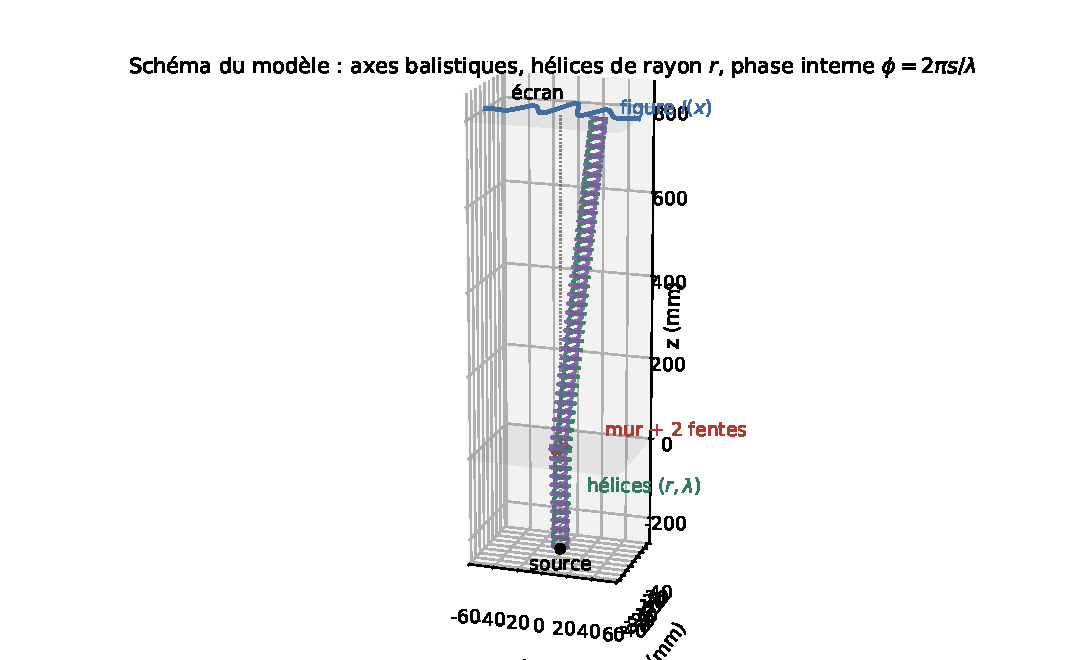
\includegraphics[width=0.84\textwidth]{figures/fig_principe.pdf}
  \caption{Schéma du modèle (échelle non contractuelle). Chaque corpuscule suit
  un axe balistique (pointillés) autour duquel il décrit une hélice de rayon $r$
  et de pas $\lambda$ portant sa phase interne $\phi = 2\pi s/\lambda$. Le point
  réel de l'hélice teste le mur (fente ou paroi) ; à l'arrivée, la détection est
  modulée par le facteur $G(x)$ construit sur les chemins virtuels des $N$ fentes,
  ce qui peint la figure d'interférence $I(x)$ sur l'écran.}
  \label{fig:principe}
\end{figure}

\begin{figure}[t]
  \centering
  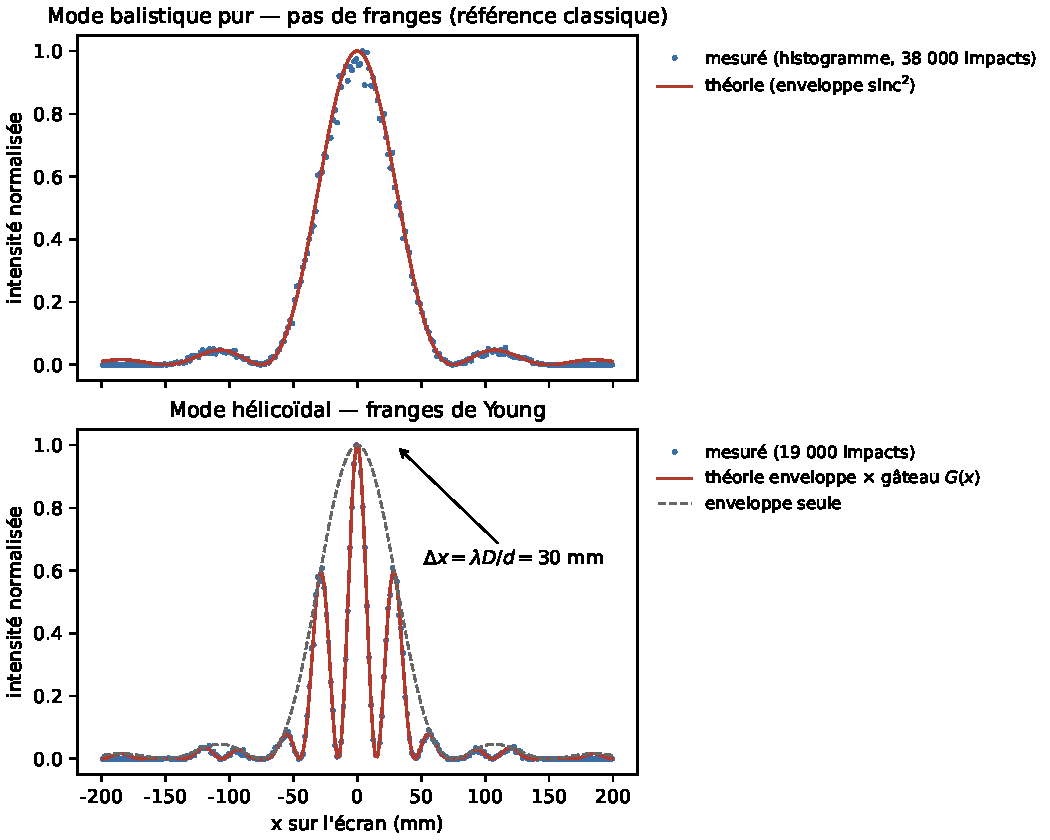
\includegraphics[width=0.88\textwidth]{figures/fig_balistique_helicoide.pdf}
  \caption{Mesures batch sur le noyau exact du simulateur (points : histogrammes
  d'impacts ; courbes : théorie du modèle, sans ajustement). \textbf{Haut} :
  mode balistique pur, $1{,}2\times10^5$ émissions, $37\,975$ impacts --- deux
  taches de diffraction, modulation $M = 0{,}004$ : aucune frange.
  \textbf{Bas} : mode hélicoïdal, $1{,}2\times10^5$ émissions, $19\,025$ impacts
  --- les franges de Young apparaissent avec $M = 0{,}994$ ; l'enveloppe seule
  (tirets) rappelle la référence balistique.}
  \label{fig:balhel}
\end{figure}

La figure~\ref{fig:balhel} porte le résultat central. En mode balistique pur ---
corpuscules ponctuels sur axes classiques, divergence de Fraunhofer au passage des
fentes --- l'histogramme d'impacts reproduit exactement la prédiction classique :
deux taches de diffraction et \emph{aucune frange}, modulation
$M = 0{,}004 \pm$ bruit de comptage. En mode hélicoïdal --- mêmes axes, mêmes
corpuscules, munis de leur phase interne et du facteur de détection $G(x)$ ---
les franges de Young apparaissent : $M = 0{,}994$. Entre les deux modes, la seule
différence est la phase interne portée par l'hélice : ni superposition d'états,
ni interaction entre corpuscules, ni onde externe.

Trois vérifications quantitatives indépendantes accompagnent cette image.
D'abord l'écart de frange : la valeur de $\dx$ qui maximise la modulation
mesurée est $\dx = 30{,}15$~mm, contre $30{,}0$~mm pour la théorie
$\lambda D /d$ --- un accord à $0{,}5\,\%$, sans paramètre ajusté. Ensuite la
fraction détectée : sur $37\,894$ corpuscules parvenus à l'écran en mode
hélicoïdal, $19\,025$ sont détectés et $18\,869$ rejetés par le gâteau, soit une
fraction détectée de $50{,}21\,\%$ contre la prédiction $\langle G \rangle = 1/N
= 50\,\%$ : le modèle est cohérent avec sa propre statistique à $0{,}2\,\%$
près. Enfin le flux : la part du faisceau qui franchit le mur vaut $31{,}6\,\%$
mesurée contre $32\,\%$ géométrique ($2 \times 1{,}6$~mm de fentes ouvertes sur
$10$~mm de faisceau) ; les $81\,713$ photons absorbés ($68{,}1\,\%$ du faisceau)
sont comptés et visibles en tant qu'éclats sur le mur dans le simulateur.

\subsection{La figure se construit corpuscule après corpuscule}

\begin{figure}[t]
  \centering
  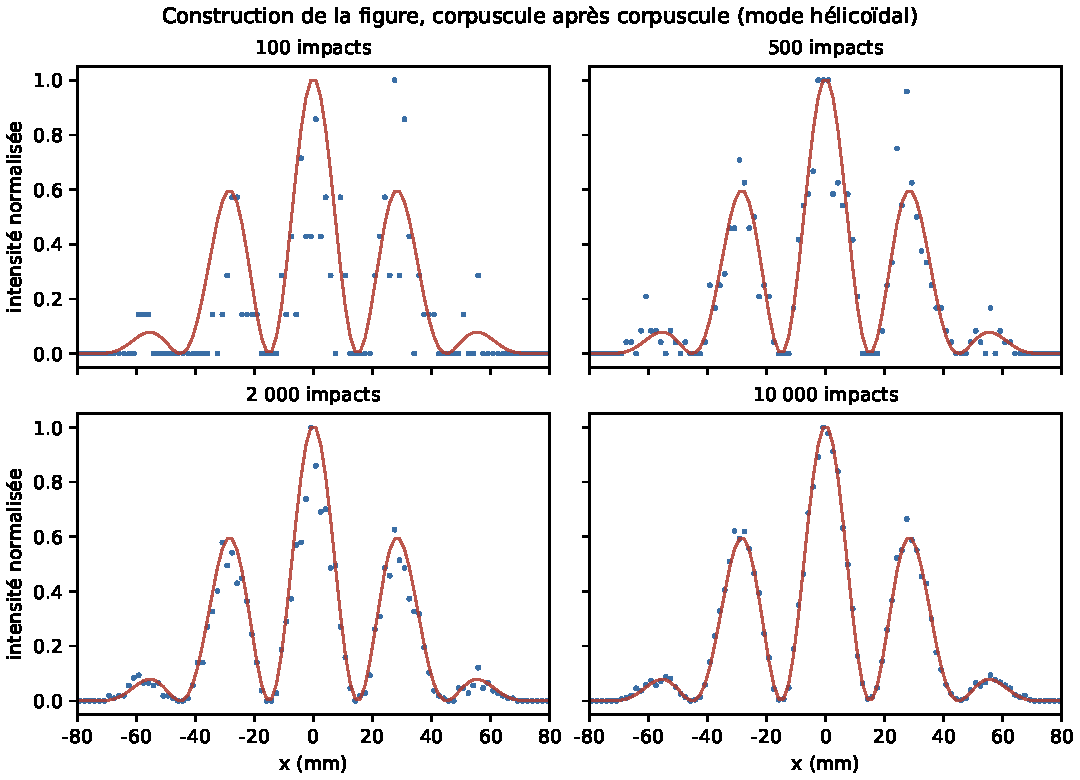
\includegraphics[width=0.95\textwidth]{figures/fig_emergence.pdf}
  \caption{Émergence de la figure (mode hélicoïdal). Clichés de l'histogramme
  d'impacts après $100$, $500$, $2\,000$ et $10\,000$ détections (points), la
  courbe théorique étant inchangée. Chaque impact individuel paraît aléatoire ;
  la distribution ne se distingue du régime balistique qu'après quelques centaines
  d'impacts, et les franges sont nettes vers $10^4$ détections --- l'analogue
  exact du film de Tonomura \cite{tonomura1989}.}
  \label{fig:emergence}
\end{figure}

La figure~\ref{fig:emergence} répond à la question « particule après
particule ». À $100$ impacts, l'histogramme est un semis apparemment désordonné
--- chaque corpuscule individualisé se comporte en tous points comme une particule
classique traverse une fente bien définie. À $10^4$ impacts, les franges sont
constituées. Il n'existe \emph{aucune étape intermédiaire} où deux corpuscules
auraient interagi : chacun ne « voit » que le mur, les fentes et l'écran. C'est la
réplique quantitative de l'expérience de Tonomura \cite{tonomura1989}, et
l'argument le plus direct contre tout mécanisme de franges par interaction
inter-corpuscules.

\subsection{Variantes : mono-fente, photon contre massif, collisions}

\begin{figure}[t]
  \centering
  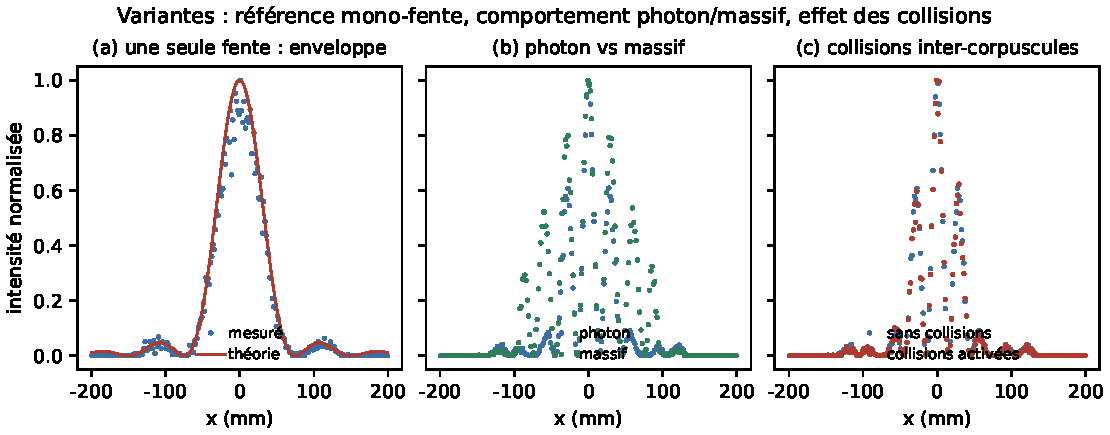
\includegraphics[width=0.98\textwidth]{figures/fig_variantes.pdf}
  \caption{Trois variantes du protocole. \textbf{(a)} Une seule fente ouverte
  ($6\times10^4$ émissions) : l'enveloppe seule, $M = 0{,}022$ --- le modèle
  retrouve automatiquement qu'une fente unique ne frange pas, car $G=1$ dès que
  $N=1$. \textbf{(b)} Photon (bleu) contre corpuscule massif (vert) : le photon
  est absorbé par la paroi ($81\,713$ absorptions, pas de halo), le massif est
  diffusé par les arêtes ($40\,732$ diffusions) et ajoute un fond diffus large,
  tandis que les franges centrales subsistent ($M = 0{,}99$).
  \textbf{(c)} Collisions inter-corpuscules activées (rayon $2$~mm, débit
  quadruplé) : $1\,355$ collisions enregistrées, $M$ passe de $0{,}994$ à
  $0{,}981$.}
  \label{fig:variantes}
\end{figure}

La figure~\ref{fig:variantes} teste trois conclusions structurelles du modèle.
\emph{(a) Mono-fente.} Avec une seule fente, $N=1$ dans l'équation~\eqref{eq:gateau}
donne $G \equiv 1$ : le modèle prédit l'enveloppe de diffraction seule, sans
franges, sans qu'on lui ait rien demandé --- et c'est ce que la mesure donne
($M = 0{,}022$). La structure multi-fentes du facteur de détection est donc bien
la seule source de franges. \emph{(b) Photon contre massif.} Le photon absorbé
par la paroi disparaît proprement : la figure reste franche, sans halo. Le
corpuscule massif, lui, est dévié par les arêtes ($40\,732$ diffusions sur
$6\times10^4$ émissions, soit $67{,}9\,\%$ du faisceau) : il survit et sème un
fond diffus sur tout l'écran, tout en laissant les franges centrales intactes
($M = 0{,}99$ contre $0{,}994$ pour le photon). Les deux comportements demandés
--- absorption franche pour le photon, déviation diffuse pour le massif --- sont
donc obtenus sans contaminer la figure d'interférence. \emph{(c) Collisions.}
Avec les collisions activées (sphères dures élastiques entre points réels des
hélices, rayon $2$~mm, $400$ corpuscules simultanés en vol), $1\,355$ collisions
sont comptées et la modulation \emph{recule} : $M = 0{,}981$ contre $0{,}994$
sans collisions. La dégradation est modeste à cette densité, mais elle est
systématique et \emph{jamais inversée} : dans ce simulateur, ajouter des
interactions entre corpuscules n'a jamais construit une frange --- elles
n'ont d'autre effet que d'éparpiller. C'est la contre-épreuve quantitative de la
section~\ref{sec:intro} : le mécanisme des franges est interne au corpuscule, et
les collisions ne font que brouiller.

\subsection{Évolution d'amplitude : franges étirées, $z$ effectif}

\begin{figure}[t]
  \centering
  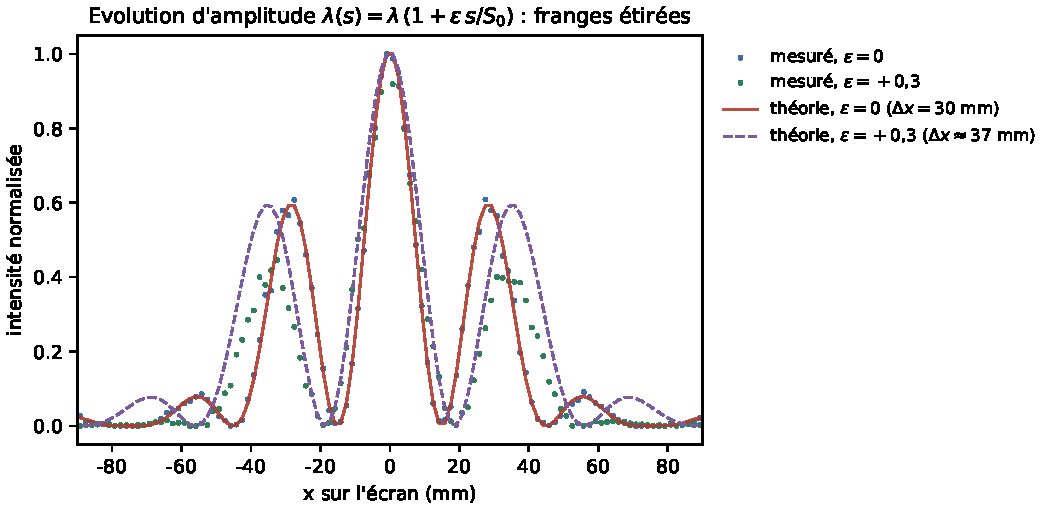
\includegraphics[width=0.88\textwidth]{figures/fig_redshift.pdf}
  \caption{Étude « redshift » ($6\times10^4$ émissions). Points bleus :
  référence $\varepsilon = 0$ ; points verts : $\varepsilon = +0{,}3$, c'est-à-dire
  $z_{\mathrm{eff}} = \varepsilon D/S_0 = 0{,}24$ et $\lambda_{\mathrm{eff}} =
  1{,}24\,\lambda$. Courbes : théorie du modèle aux mêmes paramètres. L'écart de
  frange mesuré passe de $30{,}15$~mm à $37{,}4$~mm, contre $37{,}2$~mm attendus
  ($+0{,}5\,\%$) : les franges sont étirées exactement comme le ferait un
  décalage spectral de facteur $1+z_{\mathrm{eff}}$, alors que l'énergie portée
  par chaque corpuscule est inchangée.}
  \label{fig:redshift}
\end{figure}

La figure~\ref{fig:redshift} applique la loi d'évolution d'amplitude
$\lambda(s) = \lambda(1 + \varepsilon s/S_0)$ avec $\varepsilon = +0{,}3$. Le
décalage effectif simulé vaut $z_{\mathrm{eff}} = \varepsilon D/S_0 = 0{,}24$ ;
l'écart de frange mesuré passe de $30{,}15$~mm (référence) à $37{,}4$~mm, contre
$37{,}2$~mm attendus par la longueur d'onde effective à l'écran. La structure
des franges est donc étirée du facteur $1+z_{\mathrm{eff}}$ exactement comme si
le spectre avait été décalé --- mais aucun corpuscule n'a perdu d'énergie en
chemin : seule l'horloge interne a glissé, conformément à la
loi~\eqref{eq:phaseL}. La fraction détectée reste $50{,}0\,\%$
($9\,509$ détectés, $9\,506$ rejetés) : l'étirement de phase ne change pas le
budget de détection, indice que le flux total est conservé dans le jouet
numérique. Ce point structurel --- un décalage \emph{sans perte d'énergie} ---
est le cœur de la discussion cosmologique de la section~\ref{sec:redshift}.

\begin{table}[t]
\centering\small
\caption{Récapitulatif des six runs batch (paramètres du
tableau~\ref{tab:params} sauf indication). $M$ : modulation de
frange~\eqref{eq:M} ; $\dx$ : écart de frange mesuré par maximisation de $M$
(valeur théorique entre parenthèses).}
\label{tab:runs}
\begin{tabular}{@{}l r r c l l@{}}
\toprule
Run & Émises & Détectées & $M$ & $\dx$ mesuré & Note \\
\midrule
Balistique pur   & $120\,000$ & $37\,975$ & $0{,}004$ & --- & enveloppe seule \\
Hélicoïdal       & $120\,001$ & $19\,025$ & $0{,}994$ & $30{,}15$ ($30{,}0$) & franges \\
Mono-fente       & $60\,007$  & $9\,135$  & $0{,}022$ & --- & enveloppe seule \\
Massif           & $60\,000$  & $29\,703$ & $0{,}99$  & --- & halo de diffusion \\
Redshift $\varepsilon = 0{,}3$ & $60\,002$ & $9\,509$ & $1{,}00$ & $37{,}4$ ($37{,}2$) & $z_{\mathrm{eff}} = 0{,}24$ \\
Collisions       & $60\,001$  & $8\,944$  & $0{,}981$ & --- & $1\,355$ collisions \\
\bottomrule
\end{tabular}
\end{table}

% ============================================================
\section{Lien avec le spin : la zitterbewegung}\label{sec:spin}
% ============================================================

La lecture « hélice interne $\leftrightarrow$ spin » a une histoire précise.
Schrödinger découvre dès 1930, dans les solutions de l'équation de Dirac, une
oscillation interne de l'électron à la fréquence $2mc^2/h$, la
\emph{zitterbewegung} \cite{schrodinger1930}. Hestenes propose en 1990 d'en faire
la clé de voûte de l'interprétation : l'électron y est une charge ponctuelle
décrivant une \emph{hélice} de rayon
\begin{equation}\label{eq:rz}
  r_z \;=\; \frac{\hbar}{2mc} \;=\; \frac{\hbar}{m c}\,\frac{1}{2},
\end{equation}
enroulée autour de la ligne d'univers parcourue à la vitesse moyenne de la
particule \cite{hestenes1990}. Le spin n'y est pas une propriété primitive : il
est le \emph{moment orbital du mouvement circulaire interne},
\begin{equation}\label{eq:spin}
  \lVert \vec S \rVert \;=\; m\,c\,r_z \;=\; \frac{\hbar}{2},
\end{equation}
et le moment magnétique suit, puisque la charge tournante boucle avec elle. Le
sens d'enroulement fixe l'orientation du spin.

Le simulateur de cet article est le banc d'essai minimal de cette famille
d'idées, débarrassé de la dynamique de Dirac : un corpuscule, une hélice de
rayon $r$ et de pas $\lambda$, une phase interne qui tourne comme $2\pi s/
\lambda$ --- l'« horloge interne » que de Broglie postulait dès 1927 comme
phénomène périodique au cœur du corpuscule \cite{debroglie1927} --- et un sens
d'enroulement (le paramètre \emph{spin} $\pm 1$ du simulateur, qui inverse le sens
de rotation de $\phi$). Ce que la section~\ref{sec:res} établit est précisément
le minimum dont l'interprétation zitter a besoin pour être \emph{cohérente avec
l'expérience} : une phase interne portée par le mouvement hélicoïdal suffit
statistiquement à produire la figure d'interférence, sans onde-pilote externe et
sans interaction entre corpuscules. En ce sens, le résultat du présent travail
est compatible avec, et fournit un jouet quantitatif pour, l'identification
hélice~$\leftrightarrow$~zitterbewegung~$\leftrightarrow$~spin.

Il faut être strict sur ce que le simulateur ne montre pas. D'abord,
l'échelle : $r_z = \hbar/2mc$ vaut $1{,}9\times10^{-13}$~m pour l'électron, là
où le simulateur travaille à $r = 0{,}35$~mm --- l'identification est
structurelle, l'échelle étant normalisée (section~\ref{sec:limites}).
Ensuite, la dynamique : le simulateur n'implémente pas l'équation de Dirac, ne
dérive ni le facteur gyromagnétique, ni la statistique fermionique, ni les états
de spin superposés ; le « spin » du simulateur est un sens de rotation classique.
Enfin, pour le photon, l'analogue n'est pas la zitterbewegung mais
l'\emph{hélicité} : une polarisation circulaire porte déjà un moment angulaire
$\pm\hbar$ le long de la propagation, et il n'existe pas de formulation établie
d'un photon localisé sur trajectoire hélicoïdale ; le simulateur traite donc le
photon par la seule hélice de phase, sans prétendre modéliser sa polarisation.
La position honnête est la suivante : le simulateur \emph{supporte} la
compatibilité de l'hypothèse (une phase hélicoïdale interne reproduit Young), il
ne l'\emph{établir} pas.

% ============================================================
\section{Piste de décalage vers le rouge par évolution d'amplitude}\label{sec:redshift}
% ============================================================

\subsection{Ce que la loi $\varepsilon$ réalise dans le simulateur}

Avec $\varepsilon \ne 0$, la phase cumulée $\Phi(L)$ cesse d'être linéaire
(équation~\eqref{eq:phaseL}) : tout se passe, du seul point de vue de la figure
d'interférence, comme si la longueur d'onde glissait de $\lambda$ à
$\lambda(1 + \varepsilon L/S_0)$ le long du trajet. Le simulateur mesure alors,
propagation après propagation, un décalage spectral \emph{apparent} de facteur
$1 + z_{\mathrm{eff}}$ avec $z_{\mathrm{eff}} = \varepsilon\,D/S_0$
--- linéaire en $D$, comme la loi de Hubble l'est en première approximation.
La section~\ref{sec:res} a vérifié quantitativement ce comportement
($37{,}4$~mm mesurés contre $37{,}2$~mm attendus à $z_{\mathrm{eff}} = 0{,}24$).
La question qui intéresse la cosmologie est : \emph{qu'est-ce qui distingue
structurellement ce « décalage de phase » de la « lumière fatiguée » ?}

\subsection{Distinction d'avec la lumière fatiguée de Zwicky}

La lumière fatiguée suppose que le photon \emph{perd de l'énergie} en chemin
\cite{zwicky1929} ; trois familles d'observations l'ont discréditée. Le test de
Tolman : dans un univers sans expansion, la brillance de surface des galaxies ne
peut décroître qu'en $(1+z)^{-2}$ (dilution géométrique), alors que
l'expansion prédit --- et l'observation confirme --- une décroissance proche de
$(1+z)^{-4}$ \cite{lubin2001}. La dilatation temporelle : les courbes de lumière
des supernovae Ia sont observées étirées du facteur $(1+z)$
\cite{leibundgut1996}, ce qu'un photon qui « fatigue » ne produit pas. L'absence
de flou : une perte d'énergie par diffusion élargit les images, non observées.

La variante « évolution d'amplitude » a un profil différent, et c'est ce qui
justifie de l'étudier séparément plutôt que de la rejeter par le label
« lumière fatiguée » :
\begin{itemize}[leftmargin=1.6em,itemsep=0.15em]
  \item \textbf{Pas de perte d'énergie}. Le corpuscule arrive avec l'énergie avec
        laquelle il est parti ; seul le pas de son horloge interne a glissé. La
        relation précise entre ce pas interne et la fréquence spectroscopiquement
        mesurée est une hypothèse à construire, non un acquis --- le simulateur
        est volontairement agnostique ici.
  \item \textbf{Pas de flou}. Aucune diffusion n'accompagne le glissement de
        phase : les images lointaines ne seraient pas élargies par le mécanisme
        lui-même (le simulateur le confirme : la finesse des franges est
        conservée à $\varepsilon$ non nul, $M = 1{,}00$).
  \item \textbf{Dilatation temporelle structurelle}. Si tout processus
        périodique de la source est indexé sur la phase interne du corpuscule,
        alors l'étirement des échelles de temps observées par le facteur
        $(1+z)$ est \emph{automatique} dans cette famille d'hypothèses : la
        dilatation temporelle des supernovae Ia cesse d'être un obstacle pour
        devenir une conséquence qualitative.
  \item \textbf{Le test de Tolman demeure l'obstacle central}. Le budget de
        détection du simulateur est insensible à $\varepsilon$ (fraction
        détectée $50{,}0\,\%$ à $\varepsilon = 0$ comme à $0{,}3$) : à ce niveau
        du jouet, rien ne fournit le facteur $(1+z)^{-4}$ de brillance de
        surface. Toute variante sérieuse devra soit l'engendrer, soit en
        rendre compte autrement ; c'est le test que le paramètre $\varepsilon$
        permet de formuler en laboratoire numérique.
\end{itemize}

\subsection{Échelle de l'analogie, et programme}

L'analogie est structurelle, pas quantitative. Le taux de glissement du
simulateur vaut $\varepsilon/S_0 = 3\times10^{-4}$~mm$^{-1}$ pour obtenir
$z_{\mathrm{eff}} = 0{,}24$ sur $D = 800$~mm. Le taux qui reproduirait la loi de
Hubble ($z \approx H_0 D/c$) vaut $H_0/c \approx 8\times10^{-27}$~m$^{-1}$
($H_0 \approx 70$~km/s/Mpc) : plus de vingt-cinq ordres de grandeur séparent le jouet
numérique de la moindre prétention cosmologique directe. Le rôle du simulateur
n'est pas de « faire de la cosmologie », mais d'offrir la première maquette
contrôlée du mécanisme : une commande numérique $\varepsilon$, une mesure
d'étirement, un budget d'énergie et de flux comptés --- sur lesquels on peut
greffer, étape par étape, les tests que toute variante réelle devra affronter :
linéarité $z(D)$, dilatation temporelle, finesse des images, brillance de
surface, et compatibilité avec le spectre du fond diffus cosmologique (un
étirement uniforme de toutes les longueurs d'onde préserve la forme du spectre
de Planck, ce qui est en revanche un critère redoutable pour tout mécanisme
sélectif en énergie).

% ============================================================
\section{Limites déclarées}\label{sec:limites}
% ============================================================

Le modèle est un instrument de falsification, et ses limites font partie de sa
définition. \textbf{(i)} Le facteur de détection $G(x)$ est \emph{posé},
pas dérivé d'une dynamique : le simulateur mesure sa cohérence statistique
(fraction $1/N$), il ne l'explique pas. \textbf{(ii)} La divergence post-fente
injecte l'enveloppe de Fraunhofer comme loi de tirage : le corpuscule « prend »
l'étalement que la théorie ondulatoire prédit, c'est une correspondance
construite, un paramètre et non un résultat. \textbf{(iii)} L'échelle est
normalisée ($\approx\times1000$) : aucune prétention quantitative sur les hélices
réelles (rayon $\hbar/2mc$ de la zitterbewegung) à ce stade. \textbf{(iv)} Le
comportement « massif » aux arêtes est une diffusion paramétrique, pas un
potentiel de bord dérivé. \textbf{(v)} La statistique d'écran est un empilement
d'événements indépendants : aucun effet de mémoire entre corpuscules,
contrairement aux gouttes marchantes de Couder qui gardent la trace de leur
passage \cite{couder2006,bush2015} --- ce qui, soit dit en passant, est aussi la
raison pour laquelle le simulateur ne peut pas reproduire les phénomnes de
\emph{mémoire} observés dans les analogues hydrodynamiques, et ne le cherche pas.
Enfin, rappelons que la reproduction statistique de Young par une phase interne
n'apporte \emph{aucune} évidence contre la mécanique quantique standard : elle
montre qu'un lagrangien d'information plus pauvre (trajectoire + phase) suffit
pour cette classe d'observations, ce qui est une contrainte de parcimonie sur les
interprétations, pas une réfutation.

% ============================================================
\section{Conclusions}\label{sec:ccl}
% ============================================================

Nous avons construit et validé quantitativement un simulateur stochastique de
l'expérience des fentes de Young dans lequel chaque corpuscule --- photon ou
particule massive --- suit une trajectoire hélicoïdale continue portant une phase
interne, traverse \emph{une} fente à la fois, n'interagit jamais avec ses
congénères, et dont la détection est modulée par un facteur de cohérence de phase
entre les chemins virtuels. Les résultats vont au-delà d'une reproduction
visuelle : l'écart de frange est mesuré à $0{,}5\,\%$ de la théorie
($30{,}15$ contre $30{,}0$~mm), la fraction détectée à $0{,}2\,\%$ de la
prédiction interne ($50{,}21\,\%$ contre $50\,\%$), la modulation de frange passe
de $0{,}004$ (balistique pur) à $0{,}994$ (hélicoïdal), une fente unique
retrouve l'enveloppe seule, le photon est absorbé par la paroi là où le massif
est dévié et sème un halo, les collisions inter-corpuscules ne font que
dégrader la figure, et un glissement d'amplitude $\varepsilon$ étire les franges
exactement comme un décalage spectral sans perte d'énergie ($37{,}4$ contre
$37{,}2$~mm attendus à $z_{\mathrm{eff}} = 0{,}24$).

Deux pistes de recherche en découlent, désormais dotées d'un banc d'essai
public. Pour le \textbf{spin}, le simulateur fournit le socle minimal dont
l'interprétation zitterbewegung de Hestenes a besoin : une phase hélicoïdale
interne reproduit Young ; l'identification à $r_z = \hbar/2mc$ reste qualitative
et cible future. Pour le \textbf{décalage vers le rouge}, la variante
« amplitude glissante » est structurellement distincte de la lumière fatiguée
(énergie conservée, pas de flou, dilatation temporelle automatique), mais elle
doit affronter le test de Tolman, et le simulateur offre la maquette pour
formuler ce test. Tout est reproductible en deux commandes : le code est
distribué (MIT), les mesures exportées (CSV) et chaque figure de cet article
provient du noyau exact du simulateur interactif.

% ============================================================
\appendix
\section{Reproductibilité}\label{sec:repro}
% ============================================================

Le dépôt \texttt{simulation-helicoide} contient les sources complètes. Le livrable
principal est le simulateur autonome \fichierstandalone
(double-clic, hors ligne). Les sources lisibles vivent dans \texttt{src/} :
\texttt{noyau.js} pour la physique, \texttt{rendu.js} pour la scène 3D,
\texttt{interface.js} pour les commandes. Les données exportées vivent dans
\texttt{data/} : histogrammes \texttt{mesures\_*.csv}, compteurs
\texttt{mesures\_resume.json} et métriques \texttt{mesures\_metriques.json}.
Enfin, \texttt{article/} contient la présente prépublication compilable. Les
figures et métriques de la section~\ref{sec:res} se régénèrent par :
\begin{center}\small
\begin{tabular}{@{}l@{\hspace{1.2em}}l@{}}
\texttt{node outils/mesures\_lot.js} & six runs batch ($\approx 5$~s de calcul) \\
\texttt{python3 outils/genere\_figures.py} & figures + métriques JSON \\
\texttt{python3 outils/construire\_standalone.py} & reconstruit le HTML autonome \\
\end{tabular}
\end{center}
Environnement : Node.js $\ge 14$ et Python 3 avec \texttt{numpy} et
\texttt{matplotlib} ; la compilation de l'article requiert Tectonic (LaTeX).
Le générateur de figures lit les CSV de mesures ; la courbe théorique affichée
est celle du modèle (équations~\eqref{eq:gateau}--\eqref{eq:phaseL}) évaluée aux
mêmes paramètres, sans ajustement. Licences : code et simulateur sous MIT,
documentation et article sous CC~BY~4.0 ; l'article cite le DOI du dépôt de
code lorsque celui-ci est archivé (Zenodo via GitHub, recommandé).

\begingroup
\setlength{\parskip}{0pt}
\begin{thebibliography}{99}\small
\setlength{\itemsep}{0.15em}

\bibitem{taylor1909}
G.~I. Taylor,
« Interference fringes with feeble light »,
\emph{Mathematical Proceedings of the Cambridge Philosophical Society} \textbf{15},
114--115 (1909).

\bibitem{merli1976}
P.~G. Merli, G.~F. Missiroli, G. Pozzi,
« On the statistical aspect of electron interference phenomena »,
\emph{American Journal of Physics} \textbf{44}, 306--307 (1976).

\bibitem{tonomura1989}
A. Tonomura, J. Endo, T. Matsuda, T. Kawasaki, H. Ezawa,
« Demonstration of single-electron buildup of an interference pattern »,
\emph{American Journal of Physics} \textbf{57}, 117--120 (1989),
\href{https://doi.org/10.1119/1.16104}{doi:10.1119/1.16104}.

\bibitem{bach2013}
R. Bach, D. Pope, S.-H. Liou, H. Batelaan,
« Controlled double-slit electron diffraction »,
\emph{New Journal of Physics} \textbf{15}, 033018 (2013),
\href{https://doi.org/10.1088/1367-2630/15/3/033018}{doi:10.1088/1367-2630/15/3/033018}.

\bibitem{debroglie1927}
L. de Broglie,
onde-pilote et théorie de la double solution,
communications au Congrès Solvay, Bruxelles (1927).

\bibitem{bohm1952}
D. Bohm,
« A suggested interpretation of the quantum theory in terms of ``hidden''
variables. I--II »,
\emph{Physical Review} \textbf{85}, 166--193 (1952).

\bibitem{couder2006}
Y. Couder, E. Fort,
« Single-particle diffraction and interference at a macroscopic scale »,
\emph{Physical Review Letters} \textbf{97}, 154101 (2006),
\href{https://doi.org/10.1103/PhysRevLett.97.154101}{doi:10.1103/PhysRevLett.97.154101}.

\bibitem{eddi2009}
A. Eddi, E. Fort, F. Moisy, Y. Couder,
« Unpredictable tunneling of a classical wave-particle »,
\emph{Physical Review Letters} \textbf{102}, 240401 (2009).

\bibitem{andersen2014}
A. Andersen \emph{et al.},
commentaire sur « Single-particle diffraction and interference at a macroscopic
scale », arXiv:1405.0466 (2014).

\bibitem{bush2015}
J.~W.~M. Bush,
« Pilot-wave hydrodynamics »,
\emph{Annual Review of Fluid Mechanics} \textbf{47}, 269--292 (2015).

\bibitem{schrodinger1930}
E. Schrödinger,
« Über die kräftefreie Bewegung in der relativistischen Quantenmechanik »,
\emph{Sitzungsberichte der Preußischen Akademie der Wissenschaften} (1930).

\bibitem{hestenes1990}
D. Hestenes,
« The zitterbewegung interpretation of quantum mechanics »,
\emph{Foundations of Physics} \textbf{20}, 1213--1232 (1990),
\href{https://doi.org/10.1007/BF01889466}{doi:10.1007/BF01889466}.

\bibitem{zwicky1929}
F. Zwicky,
« On the redshift of spectral lines through interstellar space »,
\emph{Proceedings of the National Academy of Sciences} \textbf{15}, 773--779 (1929),
\href{https://doi.org/10.1073/pnas.15.10.773}{doi:10.1073/pnas.15.10.773}.

\bibitem{lubin2001}
L.~M. Lubin, A. Sandage,
« The Tolman surface brightness test for the reality of the expansion »,
\emph{Astronomical Journal} \textbf{122}, 1084 (2001),
arXiv:astro-ph/0106566.

\bibitem{leibundgut1996}
B. Leibundgut \emph{et al.},
« Time dilation in the light curve of the distant type Ia supernova SN~1995K »,
\emph{Astrophysical Journal (Letters)} \textbf{466}, L21 (1996),
\href{https://doi.org/10.1086/310164}{doi:10.1086/310164}.

\end{thebibliography}
\endgroup

\end{document}


\end{document}
